\documentclass[
	a4paper, % Paper size, use either a4paper or letterpaper
	11pt, % Default font size, can also use 11pt or 12pt, although this is not recommended
	unnumberedsections, % Comment to enable section numbering
	twoside, % Two side traditional mode where headers and footers change between odd and even pages, comment this option to make them fixed
    xcolor = {dvipsnames}
]{class}

\usepackage{amssymb}
\usepackage[page,toc,titletoc,title]{appendix}
\usepackage[english]{babel}
\usepackage{csquotes}
\usepackage{float}
\usepackage{nicematrix}
\usepackage{ragged2e}
\usepackage{tikz}
\usepackage{circuitikz}
\usepackage[utf8]{inputenc}
\usepackage{filecontents}
\usepackage{listings}
\usepackage{pgfplots}
\usepackage{polski}
\usepackage{varwidth}
\usepackage{enumitem}
\usepackage{svg}
\usepackage{censor}
\pgfplotsset{compat=newest}
\usepgfplotslibrary{patchplots}

\usetikzlibrary{calc}
\usetikzlibrary{positioning}
\addbibresource{main.bib} % BibLaTeX bibliography file

\runninghead{BDD - Modèle E/A} % A shortened article title to appear in the running head, leave this command empty for no running head

\footertext{\textit{Université de Rennes - ISTIC}} % Text to appear in the footer, leave this command empty for no footer text

\setcounter{page}{1} % The page number of the first page, set this to a higher number if the article is to be part of an issue or larger work


\lstset{
    basicstyle   = \ttfamily,
    frame=tb,
    tabsize=2,
    showstringspaces=false,
    numbers=left,
    columns=fullflexible,
    breaklines=true,
    postbreak=\mbox{\textcolor{gray}{$\hookrightarrow$}\space},
}

%%%%%%%%%%%%%%%%%%%%%%%%%%%%%%%%%%%%%%%%%%%%%%%%%%%%%%%%%%%%%%%%%%%%%%%%%%%%%%%%
% Hyperef links and metadata setup
%
\hypersetup{
    unicode=true,          % non-Latin characters in Acrobat’s bookmarks
    pdftoolbar=true,        % show Acrobat’s toolbar?
    pdfmenubar=true,        % show Acrobat’s menu?
    pdffitwindow=false,     % window fit to page when opened
    pdfstartview={FitH},    % fits the width of the page to the window
    pdftitle={BDD - TP4},    % title
    pdfauthor={Alex Videcoq},     % author
    pdfsubject={BDD},   % subject of the document
    pdfnewwindow=true,      % links in new PDF window
}

%----------------------------------------------------------------------------------------
%	TITLE SECTION
%----------------------------------------------------------------------------------------

\title{BDD TP4\\---\\Modèle Entité/Association} % Article title, use manual lines breaks (\\) to beautify the layout

% Authors are listed in a comma-separated list with superscript numbers indicating affiliations
% \thanks{} is used for any text that should be placed in a footnote on the first page, such as the corresponding author's email, journal acceptance dates, a copyright/license notice, keywords, etc
\author{%
	\censor{Alex Videcoq}\textsuperscript{1}
}

% Affiliations are output in the \date{} command
\date{\footnotesize\textsuperscript{\textbf{1}}\censor{alex.videcoq}@etudiant.univ-rennes.fr}

\begin{document}

\maketitle

\begin{abstract}
    \noindent Ce document present mon travail sur le TP4 de BDD.\\
    Le but de ce TP est de modéliser une base de données à l'aide du modèle Entité/Association.\\
    Pour cela, j'ai choisi de modéliser une base de données pour le suivi et l'optimisation de la consommation d'énergie d'un réseau LoRaWAN.\\
    Ce projet me permet d'explorer la télécommunication (qui est un domaine qui m'intéresse) d'un point de vue que je n'ai pas encore abordé personnellement.
\end{abstract}

\section{Description des Entités}
\subsection{Utilisateur}
L’entité \textbf{Utilisateur} représente les individus ou organisations qui administrent et surveillent les capteurs et passerelles du réseau LoRaWAN.
\begin{itemize}
    \item \textbf{ID\_Utilisateur (PK)}: Identifiant unique de l’utilisateur.
    \item \textbf{Nom, Prénom} : Informations personnelles de l’utilisateur.
    \item \textbf{Email} : Contact de l’utilisateur.
    \item \textbf{Type\_Utilisateur} : Rôle de l’utilisateur (Administrateur, Technicien, Client, etc.).
    \item \textbf{Organisation} : Structure ou entreprise à laquelle appartient l’utilisateur.
\end{itemize}

\subsection{Capteur}
L’entité \textbf{Capteur} regroupe les capteurs connectés au réseau LoRaWAN.
\begin{itemize}
    \item \textbf{ID\_Capteur (PK)} : Identifiant unique du capteur.
    \item \textbf{Type} : Catégorie du capteur (Température, Humidité, Pression, etc.).
    \item \textbf{Modèle} : Référence du modèle de capteur utilisé.
    \item \textbf{Fréquence\_Transmission} : Intervalle d’envoi des données.
    \item \textbf{Consommation} : \'Energie consommée par le capteur (en Watt).
    \item \textbf{Date\_Installation} : Date de mise en service du capteur (timestamp Unix).
\end{itemize}

\subsection{Passerelle}
L’entité \textbf{Passerelle} représente les points relais assurant la transmission des messages entre capteurs et réseau central.
\begin{itemize}
    \item \textbf{ID\_Passerelle (PK)} : Identifiant unique de la passerelle.
    \item \textbf{Emplacement} : Position géographique de la passerelle.
    \item \textbf{État} : Statut de fonctionnement (Actif, Inactif, Maintenance).
    \item \textbf{Consommation} : Niveau d’énergie utilisée par la passerelle.
    \item \textbf{Couverture} : Zone couverte par la passerelle en kilomètres.
    \item \textbf{Source\_\'Energie} : Type d'alimentation (Solaire, Électrique, Batterie).
\end{itemize}

\subsection{Message}
L’entité \textbf{Message} stocke les données transmises par les capteurs via les passerelles.
\begin{itemize}
    \item \textbf{ID\_Message (PK)} : Identifiant unique du message.
    \item \textbf{ID\_Capteur (FK)} : Capteur émettant le message.
    \item \textbf{ID\_Passerelle (FK)} : Passerelle recevant le message.
    \item \textbf{Timestamp} : Timestamp d'\'emission du message.
    \item \textbf{Payload} : Contenu des données envoyées.
    \item \textbf{RSSI} : (\textit{Received Signal Strength Indicator}) Indicateur de puissance du signal reçu.
    \item \textbf{SNR} : (\textit{Signal-to-Noise Ratio}) Rapport signal/bruit mesuré.\\\(SNR(dB)=P_{signal\_recu}(dBm)-P_{bruit}(dBm)\)
\end{itemize}

\subsection{Optimisation Énergie}
L’entité \textbf{Opti\_Énergie} analyse et améliore la consommation énergétique des capteurs et passerelles.
\begin{itemize}
    \item \textbf{ID\_Optimisation (PK)} : Identifiant unique de l’optimisation.
    \item \textbf{ID\_Capteur} : Capteur concerné par l’optimisation.
    \item \textbf{ID\_Passerelle} : Passerelle concernée par l’optimisation.
    \item \textbf{Gain\_énergétique} : Économie d’énergie obtenue (en Watt).
    \item \textbf{Timestamp} : Date de l’étude.
    \item \textbf{Recommandation} : Actions proposées pour améliorer l’efficacité énergétique par la personne en charge de l'audit.
\end{itemize}

\section{Description des Relations}

\subsection{Relation "Gère" (Utilisateur - Capteur / Passerelle)}
\begin{itemize}
\item \textbf{Cardinalité : \((0,n) - (1.n)\)}
\item Un utilisateur peut gérer entre 0 et \(n\) capteurs/passerelles.
\item Un capteur ou une passerelle peut être géré par plusieurs utilisateurs, mais au moins un.
\end{itemize}

\subsection{Relation "Envois" (Capteur - Message)}
\begin{itemize}
\item \textbf{Cardinalité : \((1,n) - (1.1)\)}
\item Un capteur envoie plusieurs messages.
\item Un unique message ne peut être envoyé que par un seul capteur.
\end{itemize}

\subsection{Relation "Re\c{c}ois" (Passerelle - Message)}
\begin{itemize}
\item \textbf{Cardinalité : \((1,1) - (1.n)\)}
\item Un message est reçu par une seule passerelle.
\item Une passerelle peut recevoir plusieurs messages.
\end{itemize}

\subsection{Relation "Optimisation" (Capteur - Optimisation Énergie - Passerelle)}
\begin{itemize}
\item \textbf{Cardinalité : \((1,1) - (1.n) - (1,1)\)}
\item Un capteur/passerelle peut être associé à plusieurs optimisations énergétiques.
\item Une optimisation concerne un seul capteur à la fois.
\end{itemize}

\section{Exemple de requêtes}

Trouver tous les capteurs installés après 2023 :
\begin{lstlisting}[
        language=SQL,
        showspaces=false,
        basicstyle=\ttfamily,
        numbers=left,
        numberstyle=\tiny,
        commentstyle=\color{gray}
    ]
    SELECT * FROM Capteur WHERE Date_Installation > '2023-01-01';
\end{lstlisting}
\noindent
Lister les passerelles actives :
\begin{lstlisting}[
        language=SQL,
        showspaces=false,
        basicstyle=\ttfamily,
        numbers=left,
        numberstyle=\tiny,
        commentstyle=\color{gray}
    ]
    SELECT * FROM Passerelle WHERE Etat = 'Actif';
\end{lstlisting}

\noindent
Sélectionner les passerelles ayant reçu des messages avec un RSSI inférieur à -80 :
\begin{lstlisting}[
    language=SQL,
    showspaces=false,
    basicstyle=\ttfamily,
    numbers=left,
    numberstyle=\tiny,
    commentstyle=\color{gray}
]
SELECT DISTINCT P.ID_Passerelle, P.Emplacement 
FROM Passerelle P
JOIN Message M ON P.ID_Passerelle = M.ID_Passerelle
WHERE M.RSSI < -80;
\end{lstlisting}

\noindent
Identifier les capteurs avec une consommation énergétique superieure a 50W et des recommandations d'optimisation :
\begin{lstlisting}[
    language=SQL,
    showspaces=false,
    basicstyle=\ttfamily,
    numbers=left,
    numberstyle=\tiny,
    commentstyle=\color{gray}
]
SELECT C.ID_Capteur, C.Consommation, O.Recommandation
FROM Capteur C
JOIN Opti_energetique O ON C.ID_Capteur = O.ID_Capteur
WHERE C.Consommation > 50;
\end{lstlisting}

\section{Conclusion}
Ce modèle Entité/Association permet de visualiser les différentes entités et relations qui composent la base de données de suivi et d'optimisation de la consommation d'énergie d'un réseau LoRaWAN.\\
Il est possible d'ajouter des attributs supplémentaires pour chaque entité, en fonction des besoins spécifiques du projet.\\
La prochaine étape (la phase d'implementation et de deploiement) consistera à convertir ce modèle en modèle relationnel pour la création de la base de données et de pr\'eparer les requêtes SQL pour l'interrogation de la base de données.\par

\begin{figure}[H] % Two column figure (notice the starred environment)
    \begin{center}
        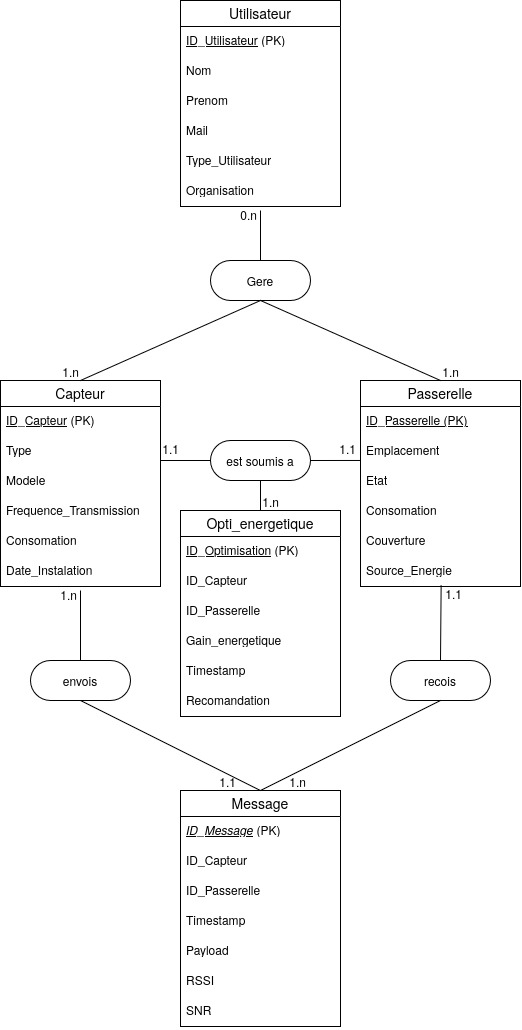
\includegraphics[height=2.5\columnwidth]{assets/LoRaWAN-db.jpg}
        \caption{Modèle Entité/Association de la base de données optimisation \'energetique LoRaWAN.}
        \label{fig:e/a LoRaWAN-db} 
    \end{center}
\end{figure}
%----------------------------------------------------------------------------------------
\end{document}